\documentclass{ctexbeamer}
\usepackage{amsmath,amssymb,amsthm,amsfonts}
\usepackage[ruled]{algorithm2e}
\usepackage{geometry}
\usepackage{ltablex}
\usepackage{bm}
\usepackage{graphicx}
\usepackage{pythonhighlight}
\usepackage{hyperref}
\usepackage{longtable}
\usepackage{multirow}
\usepackage{subcaption}
\usepackage[scr=euler]{mathalfa}
\usepackage[backend=biber]{biblatex}
\allowdisplaybreaks
\makeatletter
\renewcommand*\env@matrix[1][\arraystretch]{%
    \edef\arraystretch{#1}%
    \hskip -\arraycolsep
    \let\@ifnextchar\new@ifnextchar
    \array{*\c@MaxMatrixCols c}}
\makeatother
\renewcommand{\algorithmcfname}{}
\SetKwInput{KwIn}{输入}
\SetKwInput{KwOut}{输出}
\SetAlgoCaptionSeparator{}
\renewcommand{\thealgocf}{}
\newcommand{\epi}{\mathrm{\textbf{epi} }}
\newcommand{\diag}{\mathrm{\textbf{diag} }}
\newcommand{\tr}{\mathrm{tr}}
\newcommand{\st}{\mathrm{s.t.} \;}
\newcommand{\sign}{\mathrm{sign}}
\newcommand{\supp}{\mathrm{supp}}
\newcommand{\prox}{\mathrm{prox}}
\newcommand{\softmax}{\mathrm{softmax}}
\newcommand{\argmin}{\mathop{\arg \min }}
\newcommand{\psd}{\mathbb{P} _{S\sim \mathscr{D} ^m}}
\newcommand{\esd}{\mathbb{E} _{S\sim \mathscr{D} ^m}}
\newcommand{\pxd}{\mathbb{P} _{x\sim \mathscr{D} }}
\newcommand{\exd}{\mathbb{E} _{x\sim \mathscr{D} }}
\newcommand{\hinH}{h\in \mathscr{H} }
\newcommand{\norm}[1]{\left\lVert #1\right\rVert}
\newcommand{\inprod}[1]{\left\langle #1\right\rangle}
\usefonttheme{serif}
% 选择主题
\usetheme{Berlin}
\addbibresource{ref.bib}

\title{Training Data Selection Methods for Deep Learning Based on Diversity-Aware Heuristic Strategies}
\author{\begin{tabular}{cccc}
    刘子宁 & 雷纯熙 & 张蔚峻 & 伍思亦 \\
    2401110050 & 2401110045 & 2401110059 & 2401110071 
\end{tabular}}
\institute{}
\date{}

% 禁用顶部的标题栏
\setbeamertemplate{headline}{}
\setbeamertemplate{footline}{}

% 自定义底部的内容
% \setbeamertemplate{footline}
% {
%   \hbox{%
%     \begin{beamercolorbox}[wd=.333333\paperwidth,ht=2.25ex,dp=1ex,center]{author in head/foot}%
%       \usebeamerfont{author in head/foot}\insertshortauthor
%     \end{beamercolorbox}%
%     \begin{beamercolorbox}[wd=.333333\paperwidth,ht=2.25ex,dp=1ex,center]{title in head/foot}%
%       \usebeamerfont{title in head/foot}\insertshorttitle
%     \end{beamercolorbox}%
%     \begin{beamercolorbox}[wd=.333333\paperwidth,ht=2.25ex,dp=1ex,right]{date in head/foot}%
%       \usebeamerfont{date in head/foot}\insertshortdate{}\hspace*{2em}
%     \end{beamercolorbox}}%
%   \vskip0pt%
% }

\begin{document}

% 标题页
\begin{frame}
  \titlepage
\end{frame}

% 目录
\begin{frame}{Contents}
  \tableofcontents
\end{frame}

% 第一节
\section{Introduction}
\begin{frame}{Introduction}
    Efficient training of deep learning models often requires selective data sampling to accelerate convergence and enhance generalization. This research investigates data selection methods informed by heuristic strategies, which leverage model-specific metrics to prioritize training samples. The objective is to explore how different selection strategies impact model performance and efficiency in large-scale training tasks.
\end{frame}

% 第二节
\section{Problem Setting}
\begin{frame}{Problem Setting}
    Given a training dataset $\mathcal{D} = \{(x_i, y_i)\}_{i=1}^N$ and a model $f_\theta(x)$ parameterized by $\theta$, the loss function $L(\theta, x, y)$ is used to measure the discrepancy between predictions and true labels. The problem can be defined as:

    \[
    \min_{\theta} \frac{1}{|\mathcal{B}|} \sum_{(x, y) \in \mathcal{B}} L(\theta, x, y),
    \]
    
    where $\mathcal{B} \subseteq \mathcal{D}$ is the selected batch of training samples. The challenge is to construct $\mathcal{B}$ based on criteria that optimize training efficiency while ensuring diversity in the selected data. 
    
    Key considerations:
    \begin{itemize}
        \item Samples should be selected to maximize their contribution to the training process.
        \item The selection strategy must balance focus on challenging examples and coverage of the dataset's diversity.
    \end{itemize}
\end{frame}

\section{Methods}
\begin{frame}[allowframebreaks]{Methods}
    We propose to evaluate the following training data selection strategies:
    \begin{enumerate}
        \item \textbf{High-Loss Selection}\cite{Loss}: Samples are chosen based on their loss values $L(\theta, x, y)$. Let $\mathcal{B}$ be the top $k$ samples ranked by $L(\theta, x, y)$.
        \item \textbf{High-Gradient Selection}\cite{Gradient}: Samples are prioritized based on the norm of the gradient of the loss with respect to model parameters:
        \[\|\nabla_\theta L(\theta, x, y)\|.\]
        \item \textbf{High-Influence Selection}\cite{Influence}: Samples are selected based on the influence of the input on the loss, calculated as:
        \[\left\|\frac{\partial L(\theta, x, y)}{\partial x}\right\|.\]
        \item \textbf{Random Sampling (Baseline)}: Samples are randomly selected from $\mathcal{D}$ without considering loss or gradient metrics.
    \end{enumerate}

    We conducted experiments comparing several dataset pruning strategies on the MNIST and CIFAR10 datasets.
    \begin{itemize}
        \item Random: Randomly select samples
        \item Loss: Select samples with the highest loss values on the surrogate model
        \item Loss-Grad: Select samples with the largest loss gradient norms on the surrogate model
        \item EL2N\cite{paul2021deep}: Select samples with the largest error vector norms on the surrogate model
    \end{itemize}
\end{frame}

\begin{frame}[allowframebreaks]{EL2N Introduction}
The Error L2-Norm (EL2N) scoring method is a data selection strategy used in deep learning to identify important training examples early in the training process. This method computes a score for each training sample based on its prediction error vector's L2 norm.

The EL2N score for a training sample \((x, y)\) is defined as:
\[\text{EL2N}(x, y) = \mathbb{E} \| p(w_t, x) - y \|^2\]
where:
\begin{itemize}
  \item $p(w_t, x)$ is the predicted probability vector output by the model for input $x$ at training step $t$.
  \item $y$ is the one-hot encoded true label of the sample.
  \item $\mathbb{E}$ denotes the expectation, typically computed by averaging over multiple model initializations.
\end{itemize}

The EL2N score has several key applications:
\begin{itemize}
  \item \textbf{Data Pruning}: Removing samples with low EL2N scores early in training reduces the dataset size while maintaining or even improving model performance.
  \item \textbf{Noise Detection}: High EL2N scores can indicate noisy or mislabeled examples.
  \item \textbf{Generalization Improvement}: Pruning unimportant samples helps avoid overfitting and enhances test accuracy.
\end{itemize}

Unlike methods such as the "forgetting score," which requires monitoring the entire training process, EL2N uses only local prediction errors calculated in the first few epochs. This makes EL2N computationally efficient while delivering comparable or superior performance.
\end{frame}

\section{Numerical Experiment}
\begin{frame}{Numerical Experiment}
    \begin{itemize}
        \item \textbf{Datasets}: CIFAR-10 and MNIST for image classification tasks.
        \item \textbf{Model Architectures}: \begin{itemize}
            \item For MNIST, we use CNN(2 convolution layers+2 fully connected layers) with SGD optimizer.
            \item For CIFAR-10, we use ResNet18 with SGD optimizer.
        \end{itemize}
        \item \textbf{Evaluation Metrics}: Final model accuracy on test data.
    \end{itemize}
\end{frame}

\begin{frame}{Numerical Experiment}
    The 10 samples with the highest loss in the MNIST dataset:
    \begin{center}
        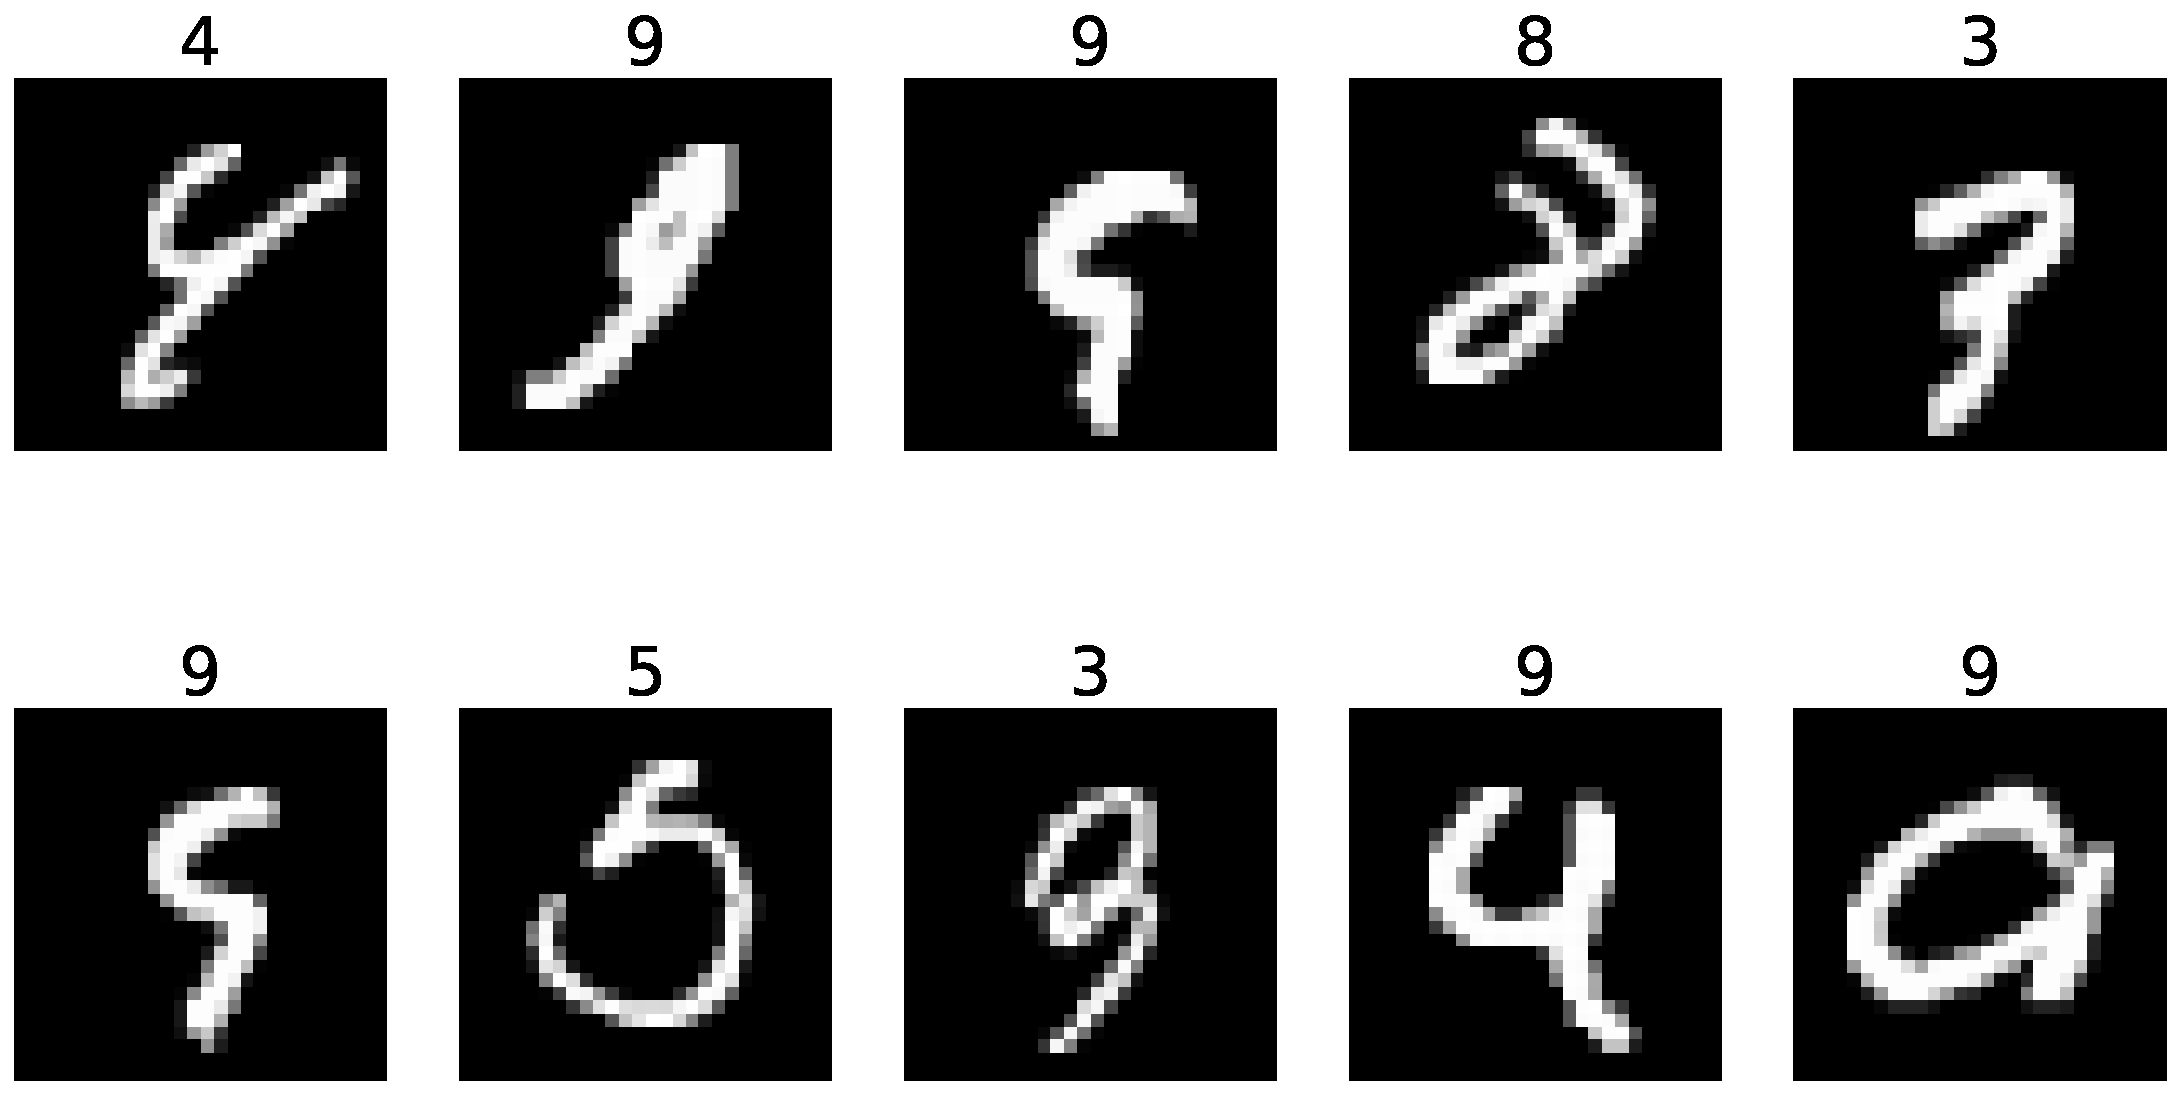
\includegraphics[width=0.6\textwidth]{../images/mnist_hard_samples.pdf}
    \end{center}
    
    Repetition rate for the first 10000 samples and last 10000 samples (\(S_1\):Loss,\(S_2\):Loss-Grad,\(S_3\):EL2N):
    \begin{itemize}
        \item \(R_{\text{first} }(S_1,S_2)=96.78\%,R_{\text{last} }(S_1,S_2)=95.01\%\)
        \item \(R_{\text{first} }(S_2,S_3)=96.45\%,R_{\text{last} }(S_2,S_3)=95.89\%\)
        \item \(R_{\text{first} }(S_1,S_3)=97.68\%,R_{\text{last} }(S_1,S_3)=96.32\%\)
    \end{itemize}
\end{frame}

\begin{frame}{Numerical Experiment}
    Training with different purning ratio:
    \begin{center}
        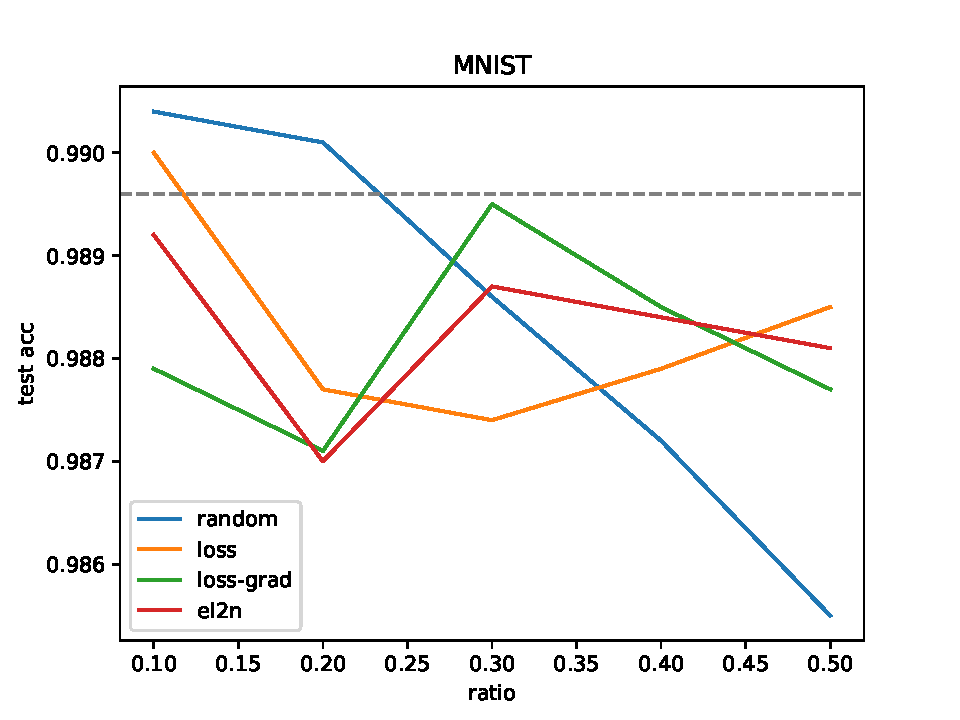
\includegraphics[width=0.45\textwidth]{../images/mnist_ratio.pdf}
        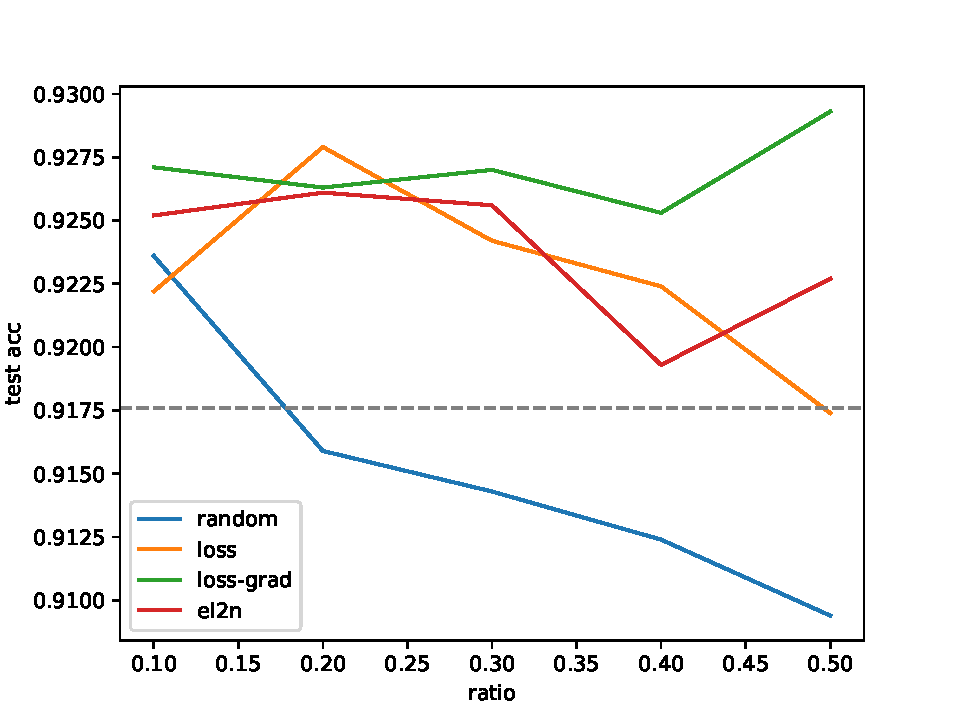
\includegraphics[width=0.45\textwidth]{../images/cifar10_ratio.pdf}
    \end{center}
\end{frame}

\begin{frame}{Numerical Experiment}
    Pruning after different pre-training epochs:
    \begin{center}
        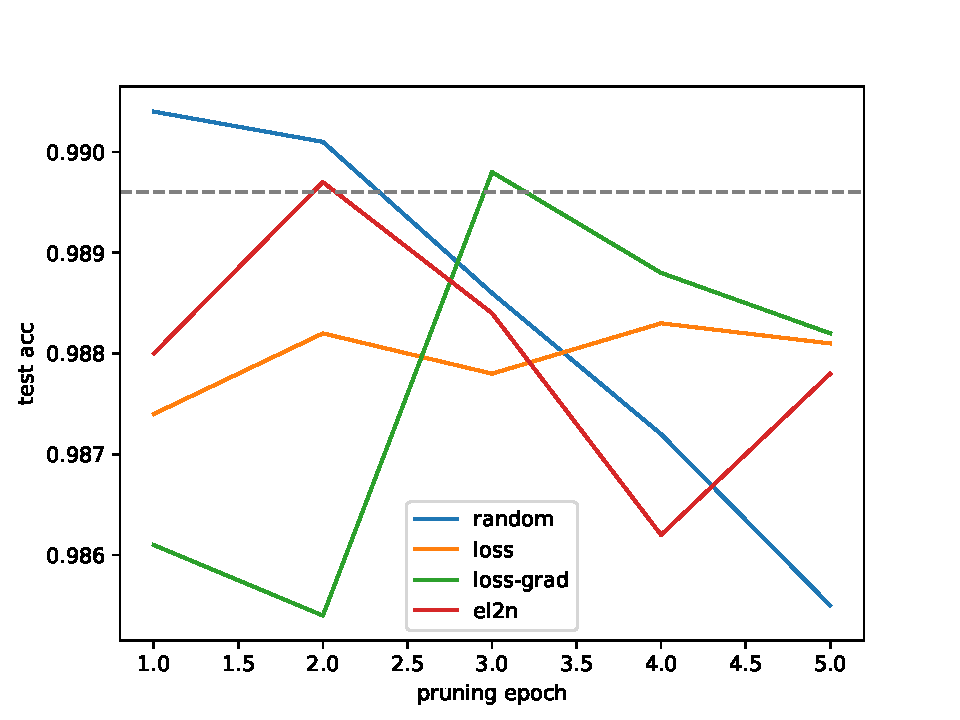
\includegraphics[width=0.45\textwidth]{../images/mnist_pruning.pdf}
        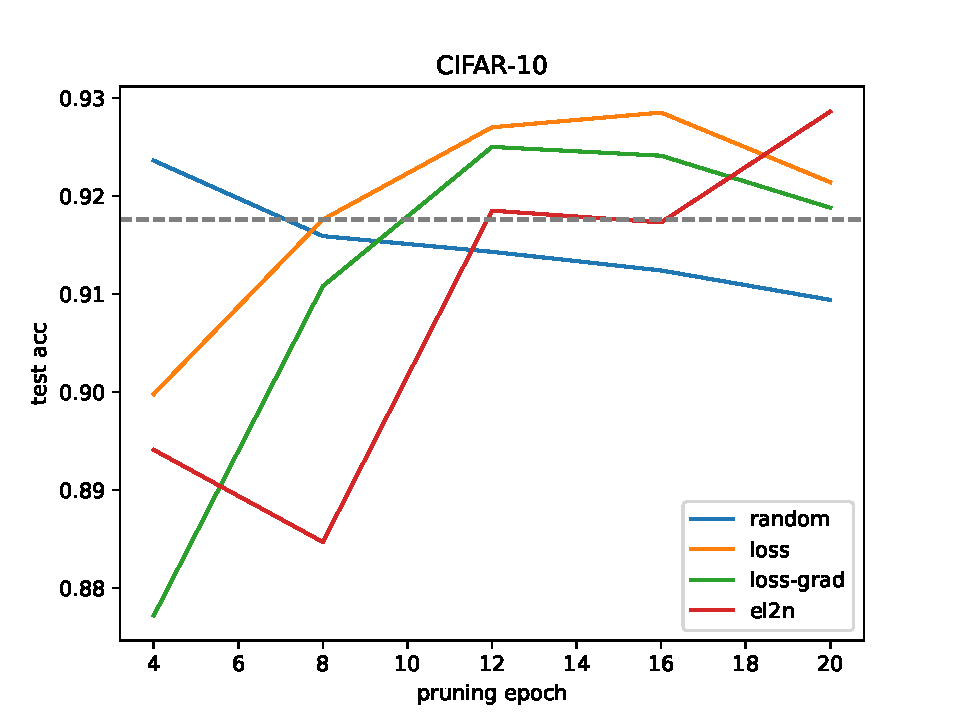
\includegraphics[width=0.45\textwidth]{../images/cifar10_pruning.pdf}
    \end{center}
\end{frame}

\section{Conclusion}
\begin{frame}{Conclusion}
    Through numerical experiments, we can draw the following conclusions:
    \begin{itemize}
        \item In smaller datasets, randomness has a greater impact on the results.
        \item The selected data by existing methods have high similarity.
        \item If the pruning ratio is not too large, choosing "hard" examples well be more benificial.
    \end{itemize}
\end{frame}

% 参考文献
\section{References}
\begin{frame}{References}
    \printbibliography
\end{frame}

\end{document}
